\documentclass[conference]{IEEEtran}
\IEEEoverridecommandlockouts
% The preceding line is only needed to identify funding in the first footnote. If that is unneeded, please comment it out.
\usepackage{cite}
\usepackage{amsmath,amssymb,amsfonts}
\usepackage{algorithmic}
\usepackage{graphicx}
% Search for figures in current folder and architecture/ subfolder
\graphicspath{{./}{architecture/}}
\usepackage{textcomp}
\usepackage{xcolor}
\def\BibTeX{{\rm B\kern-.05em{\sc i\kern-.025em b}\kern-.08em
    T\kern-.1667em\lower.7ex\hbox{E}\kern-.125emX}}
\begin{document}

\title{TripSync: An Integrated Platform for Student Commute-Sharing and Academic Collaboration in Higher Education}

\author{\IEEEauthorblockN{Varun Gupta}
\IEEEauthorblockA{\textit{Department of Artificial Intelligence and Data Science} \\
\textit{Dwarkadas J. Sanghvi College of Engineering}\\
Mumbai, India \\
varunygupta123@gmail.com}
\and
\IEEEauthorblockN{Kavish Shah}
\IEEEauthorblockA{\textit{Department of Artificial Intelligence and Data Science} \\
\textit{Dwarkadas J. Sanghvi College of Engineering}\\
Mumbai, India \\
kavishshah@gmail.com}
\and
\IEEEauthorblockN{Harsh Chandramania}
\IEEEauthorblockA{\textit{Department of Artificial Intelligence and Data Science} \\
\textit{Dwarkadas J. Sanghvi College of Engineering}\\
Mumbai, India \\
harshchandramania@gmail.com}
\and
\IEEEauthorblockN{Paarth Gala}
\IEEEauthorblockA{\textit{Department of Artificial Intelligence and Data Science} \\
\textit{Dwarkadas J. Sanghvi College of Engineering}\\
Mumbai, India \\
paarthgala@gmail.com}
}

\maketitle

\begin{abstract}
The daily commuting challenges faced by college students reveal significant inefficiencies in current transportation and communication systems within higher education environments. Personal observations from metro station to college commutes demonstrate that students frequently travel alone or in small groups, facing high transportation costs ranging from Rs.60-80 during regular hours to Rs.110 during peak times, while struggling to find available shared transportation options. This paper presents TripSync, an integrated platform addressing these real-world challenges by connecting verified college students for safe, cost-effective ride-sharing while simultaneously facilitating academic collaboration and institutional communication. The platform emerges from identified pain points including expensive solo travel, time-consuming auto-rickshaw searches, inefficient faculty-student coordination for placement assistance, delayed senior-junior collaboration for research projects, and costly manual committee recruitment through class visits and poster campaigns. TripSync leverages React Native for cross-platform mobile development and Node.js for backend services, incorporating intelligent matching algorithms that enable students to connect with trusted college peers for transportation while providing structured channels for academic mentorship, committee recruitment, and faculty assistance requests. Through systematic analysis of current communication fragmentation and transportation inefficiencies, this research demonstrates that TripSync can significantly reduce individual commuting costs by 40-60\%, enhance safety through verified college ecosystems, and improve academic collaboration efficiency by replacing manual processes with targeted digital campaigns similar to modern app-based advertising strategies. The platform's unique integration addresses multiple interconnected student needs through a single, verified, college-specific solution.
\end{abstract}

\begin{IEEEkeywords}
student transportation, academic collaboration, service-learning, mobile application, peer-to-peer sharing, educational technology
\end{IEEEkeywords}

\section{Introduction}

Higher education institutions face persistent challenges in facilitating effective student collaboration and providing affordable, safe transportation solutions. Real-world observations from daily college commutes reveal the extent of these challenges: students traveling alone from metro stations to college face transportation costs ranging from Rs.60-80 during regular hours, escalating to Rs.110 during peak times, while simultaneously struggling to locate available auto-rickshaws in crowded urban environments \cite{ref1}\cite{ref2}. These individual experiences reflect broader systemic issues where traditional approaches to academic mentorship and commute management operate in isolated silos, creating inefficiencies and missed opportunities for student engagement.

"What began as a struggle to find affordable transport from the metro to campus revealed a deeper set of challenges in how students and faculty connect, collaborate, and communicate." This observation encapsulates the interconnected nature of challenges facing modern higher education, where transportation difficulties serve as a lens through which broader institutional communication and collaboration inefficiencies become apparent.

The fragmentation of current coordination systems manifests in several critical areas affecting daily student life. Students depend on informal WhatsApp groups for ride coordination, which lack safety verification and structured oversight, often resulting in time-consuming searches for transportation and higher individual costs \cite{ref3}\cite{ref4}. Academic collaboration typically happens through general-purpose applications that were not designed for educational environments, while faculty members seeking student assistance for placement activities or project work face tedious individual messaging and overwhelming response management \cite{ref5}\cite{ref6}. Committee recruitment and event promotion continue to rely on manual methods such as class-to-class visits and physical poster campaigns, representing significant expenses and inefficient resource allocation compared to modern targeted digital advertising approaches used by platforms like Zomato and Duolingo \cite{ref7}\cite{ref8}.

The disconnect between senior and junior students presents additional collaboration barriers. Seniors requiring junior assistance for research paper writing or other academic tasks face delays and difficulty identifying suitable candidates due to lack of structured platforms for academic partnerships \cite{ref9}\cite{ref10}. This fragmentation forces students to navigate multiple disconnected systems while committees and faculty struggle with reach, engagement, and cost-effective communication strategies \cite{ref11}\cite{ref12}.

Research consistently demonstrates that students overwhelmingly prefer quick, text-based mobile communication over email and video calls, yet existing platforms fail to leverage these communication preferences in educational contexts while addressing practical daily challenges like transportation coordination \cite{ref13}\cite{ref14}. This gap represents a substantial opportunity to develop technology solutions that simultaneously address logistical challenges while fostering meaningful educational experiences through mobile-first, integrated approaches.

TripSync emerges as a comprehensive response to these interconnected challenges, providing an integrated platform that combines intelligent commute-sharing with robust academic collaboration, mentorship coordination, and committee recruitment features. By leveraging college ID authentication, specialized matching algorithms, and text-first communication design, TripSync creates a trusted ecosystem where students can safely coordinate transportation while engaging in structured academic partnerships, addressing the real-world pain points observed in daily college life.

This research presents the design, implementation, and evaluation of TripSync, demonstrating its potential to transform both student transportation and academic collaboration within higher education institutions. The platform's innovative approach addresses critical gaps identified through direct observation of student challenges while providing measurable benefits in cost reduction, safety enhancement, and educational outcomes through unified, student-centered digital solutions.

\section{Literature Review}

The development of TripSync is grounded in extensive research across service-learning management, digital collaboration platforms, and student engagement technologies. This literature review examines the current state of campus communication and collaboration while identifying critical gaps that justify an integrated platform approach.

\subsection{Current State of Campus Communication and Collaboration}

Campus communication and collaboration currently rely on a patchwork of tools and outdated practices. For ride-sharing, students often depend on informal WhatsApp groups or word of mouth, which lack safety checks and structured coordination \cite{ref15}\cite{ref16}. Academic collaboration typically happens through general-purpose apps like Google Docs or Slack, while mentoring and peer support are either unstructured or limited to small faculty-run programs \cite{ref17}\cite{ref1}. Committee recruitment and event promotion remain largely manual—student organizers go class-to-class or rely on posters around campus, which is inefficient, time-consuming, and environmentally wasteful \cite{ref2}\cite{ref3}.

At the same time, students overwhelmingly prefer quick, text-based mobile communication, which consistently outperforms email and avoids the barriers of video calls \cite{ref4}\cite{ref5}. This reality highlights the need for an integrated, student-centered platform that fits into existing communication habits while reducing reliance on fragmented and outdated systems \cite{ref6}\cite{ref7}. Research consistently demonstrates that modern students engage more effectively through mobile-first, text-based interfaces that support both synchronous and asynchronous communication modalities \cite{ref8}\cite{ref9}.

\subsection{Gaps and Justification for Integrated Solutions}

The major limitation of current approaches is their lack of integration. Transportation, project work, mentoring, and event promotion are all treated separately, forcing students to juggle multiple channels while committees and faculty struggle with reach and engagement \cite{ref10}\cite{ref11}. Existing digital tools rarely address same-college ecosystems, where identity verification and trust are critical for safe and effective collaboration \cite{ref12}\cite{ref13}. Moreover, recruitment practices remain stuck in physical modes of outreach, despite students already being immersed in mobile-first environments \cite{ref14}.

There is also little support for transparent, profile-driven trust mechanisms such as resumes and verification systems, which could improve collaboration and mentorship matching \cite{ref15}\cite{ref16}. Current service-learning management platforms, while effective for logistics, inadequately address the relational and mentoring aspects crucial for meaningful academic collaboration \cite{ref17}\cite{ref1}. The fragmentation of communication channels results in missed opportunities for cross-functional student interactions that could enhance both academic and social outcomes \cite{ref2}\cite{ref3}.

TripSync addresses these gaps by combining ride-sharing, academic collaboration, mentorship, and committee recruitment into a single, text-first platform. By replacing posters with digital announcements, class visits with in-app subscriptions, and fragmented groups with verified profiles, TripSync aligns with real student behavior while offering a scalable model for safer, more efficient, and more inclusive campus collaboration \cite{ref4}\cite{ref5}. The platform's integrated approach recognizes that student needs are interconnected and require holistic solutions rather than isolated point solutions \cite{ref6}\cite{ref7}.

\section{Problem Statement}

The current landscape of student transportation and academic collaboration in higher education presents several interconnected challenges that significantly impact student experience, learning outcomes, and institutional efficiency. These problems, observed through direct experience and systematic analysis of daily college operations, manifest across multiple dimensions of student life and require comprehensive solutions.

\subsection{High Transportation Costs and Inefficient Coordination}

Daily commuting from metro stations to college campuses reveals significant economic burdens on students. Individual transportation costs range from Rs.60-80 during regular hours, escalating to Rs.90-100 during peak periods, and reaching Rs.110 for return journeys from college to metro stations \cite{ref8}\cite{ref9}. These costs become particularly prohibitive when students travel alone, which frequently occurs due to lack of coordination mechanisms among college peers traveling similar routes.

The time spent searching for available auto-rickshaws increases during peak hours when public transport is overcrowded or unavailable, compounding both cost and time inefficiencies \cite{ref10}\cite{ref11}. Students often observe multiple college peers traveling the same route individually or in small groups of two, representing missed opportunities for cost-sharing and efficient transportation coordination \cite{ref12}\cite{ref13}.

\subsection{Inefficient Faculty-Student Communication Systems}

Faculty members seeking student assistance for placement activities, research projects, or administrative tasks face significant communication challenges through current systems. WhatsApp group messaging results in overwhelming responses that require individual replies, creating time-consuming and tedious coordination processes \cite{ref14}\cite{ref15}. The lack of structured application and screening mechanisms leads to mismatched expectations and inefficient resource allocation.

Current communication methods fail to provide faculty with adequate information about student qualifications, interests, and availability, resulting in suboptimal matching for collaborative opportunities \cite{ref16}\cite{ref17}. This creates delays in critical activities such as placement coordination and academic project assistance.

\subsection{Barriers to Senior-Junior Academic Collaboration}

Senior students requiring assistance from juniors for research paper writing, project development, or other academic tasks face significant challenges in identifying and connecting with suitable candidates \cite{ref1}\cite{ref2}. The absence of structured platforms for academic partnerships results in delays, missed opportunities, and uninformed decision-making regarding junior student capabilities and compatibility.

Current informal networking approaches provide insufficient information for seniors to make informed decisions about potential collaborators, leading to project delays and suboptimal academic partnerships \cite{ref3}. The lack of transparent profile and credential sharing mechanisms hinders effective matching between senior project needs and junior skills and interests.

\subsection{Costly and Inefficient Committee Recruitment Methods}

College committees continue to rely on manual recruitment strategies including class-to-class visits and physical poster campaigns, representing significant expenses and inefficient resource allocation \cite{ref4}. These methods contrast sharply with modern targeted digital advertising approaches used by successful platforms like Zomato and Duolingo, which achieve higher engagement rates at lower costs.

Manual recruitment methods fail to leverage student preferences for digital communication, result in limited reach and engagement, and represent poor use of committee resources that could be redirected toward programmatic activities \cite{ref5}. The environmental impact of poster-based campaigns also contradicts institutional sustainability goals while failing to achieve effective targeting and engagement metrics available through digital platforms.

\section{Objectives of TripSync}

TripSync is designed to address the identified challenges through a comprehensive platform that integrates transportation coordination with academic collaboration, mentorship facilitation, and committee recruitment. The platform's objectives are structured around four primary goals that collectively transform the student experience while supporting institutional educational and sustainability objectives.

\subsection{Affordable and Reliable Commute Solutions}

The primary objective is to provide students with affordable, safe, and reliable commute-sharing options that significantly reduce individual transportation costs while promoting environmental sustainability \cite{ref6}\cite{ref7}. By facilitating ride-sharing among verified students, TripSync enables cost distribution across multiple participants, making daily commuting more economically accessible while reducing the overall carbon footprint of institutional transportation patterns.

The platform aims to achieve cost reductions of 40-60\% compared to individual transportation or commercial ride-sharing services, while maintaining reliability through systematic matching algorithms, user accountability mechanisms, and integrated safety protocols \cite{ref8}\cite{ref9}.

\subsection{Verified Student-Only Ecosystem with Enhanced Safety}

TripSync creates a trusted, college-verified ecosystem that ensures all participants are authenticated students from recognized educational institutions \cite{ref10}\cite{ref11}. Through integration with college ID systems and institutional email verification, the platform provides a level of safety and trust that commercial alternatives cannot offer, addressing specific concerns about anonymous ride-sharing services.

This verification system incorporates transparent, profile-driven trust mechanisms including academic credentials and peer ratings, fostering a sense of community and shared institutional identity among users \cite{ref12}\cite{ref13}. The platform's design prioritizes student privacy while maintaining necessary oversight for safety and accountability through institutional partnerships.

\subsection{Integrated Academic and Social Collaboration Enhancement}

A key objective is to facilitate meaningful academic collaboration between students of different academic levels through integrated community features that replace fragmented communication systems \cite{ref14}\cite{ref15}. TripSync provides structured spaces for research paper exchange, academic mentoring, placement guidance, collaborative project development, and committee recruitment, all accessible through text-first mobile interfaces that align with student communication preferences.

The platform aims to increase inter-level academic interactions by 200-300\% compared to traditional informal networks, while providing faculty and administrators with tools to monitor and support these collaborations \cite{ref16}\cite{ref17}. By replacing manual poster-based recruitment with digital announcements and class visits with in-app subscriptions, TripSync creates scalable, efficient communication channels.

\subsection{Unified Digital Campus Communication}

TripSync promotes the replacement of outdated communication practices with a comprehensive digital platform that serves as a central hub for campus collaboration \cite{ref1}\cite{ref2}. The objective is to consolidate fragmented communication channels—from informal WhatsApp groups to physical bulletin boards—into a single, institution-specific platform that maintains community identity while enabling efficient information sharing.

The platform tracks and reports engagement metrics, communication efficiency, and collaboration success rates, providing institutions with data to support digital transformation initiatives while encouraging continued platform adoption and community development \cite{ref3}.

\section{System Design and Features}

TripSync architecture is designed as a comprehensive mobile platform that seamlessly integrates transportation coordination with academic collaboration features. The system employs a modular design approach that ensures scalability, maintainability, and extensibility while providing intuitive user experiences across all functional areas. The overall system architecture is depicted in Fig.~\ref{fig:system_architecture}.

\begin{figure}[!htbp]
  \centering
  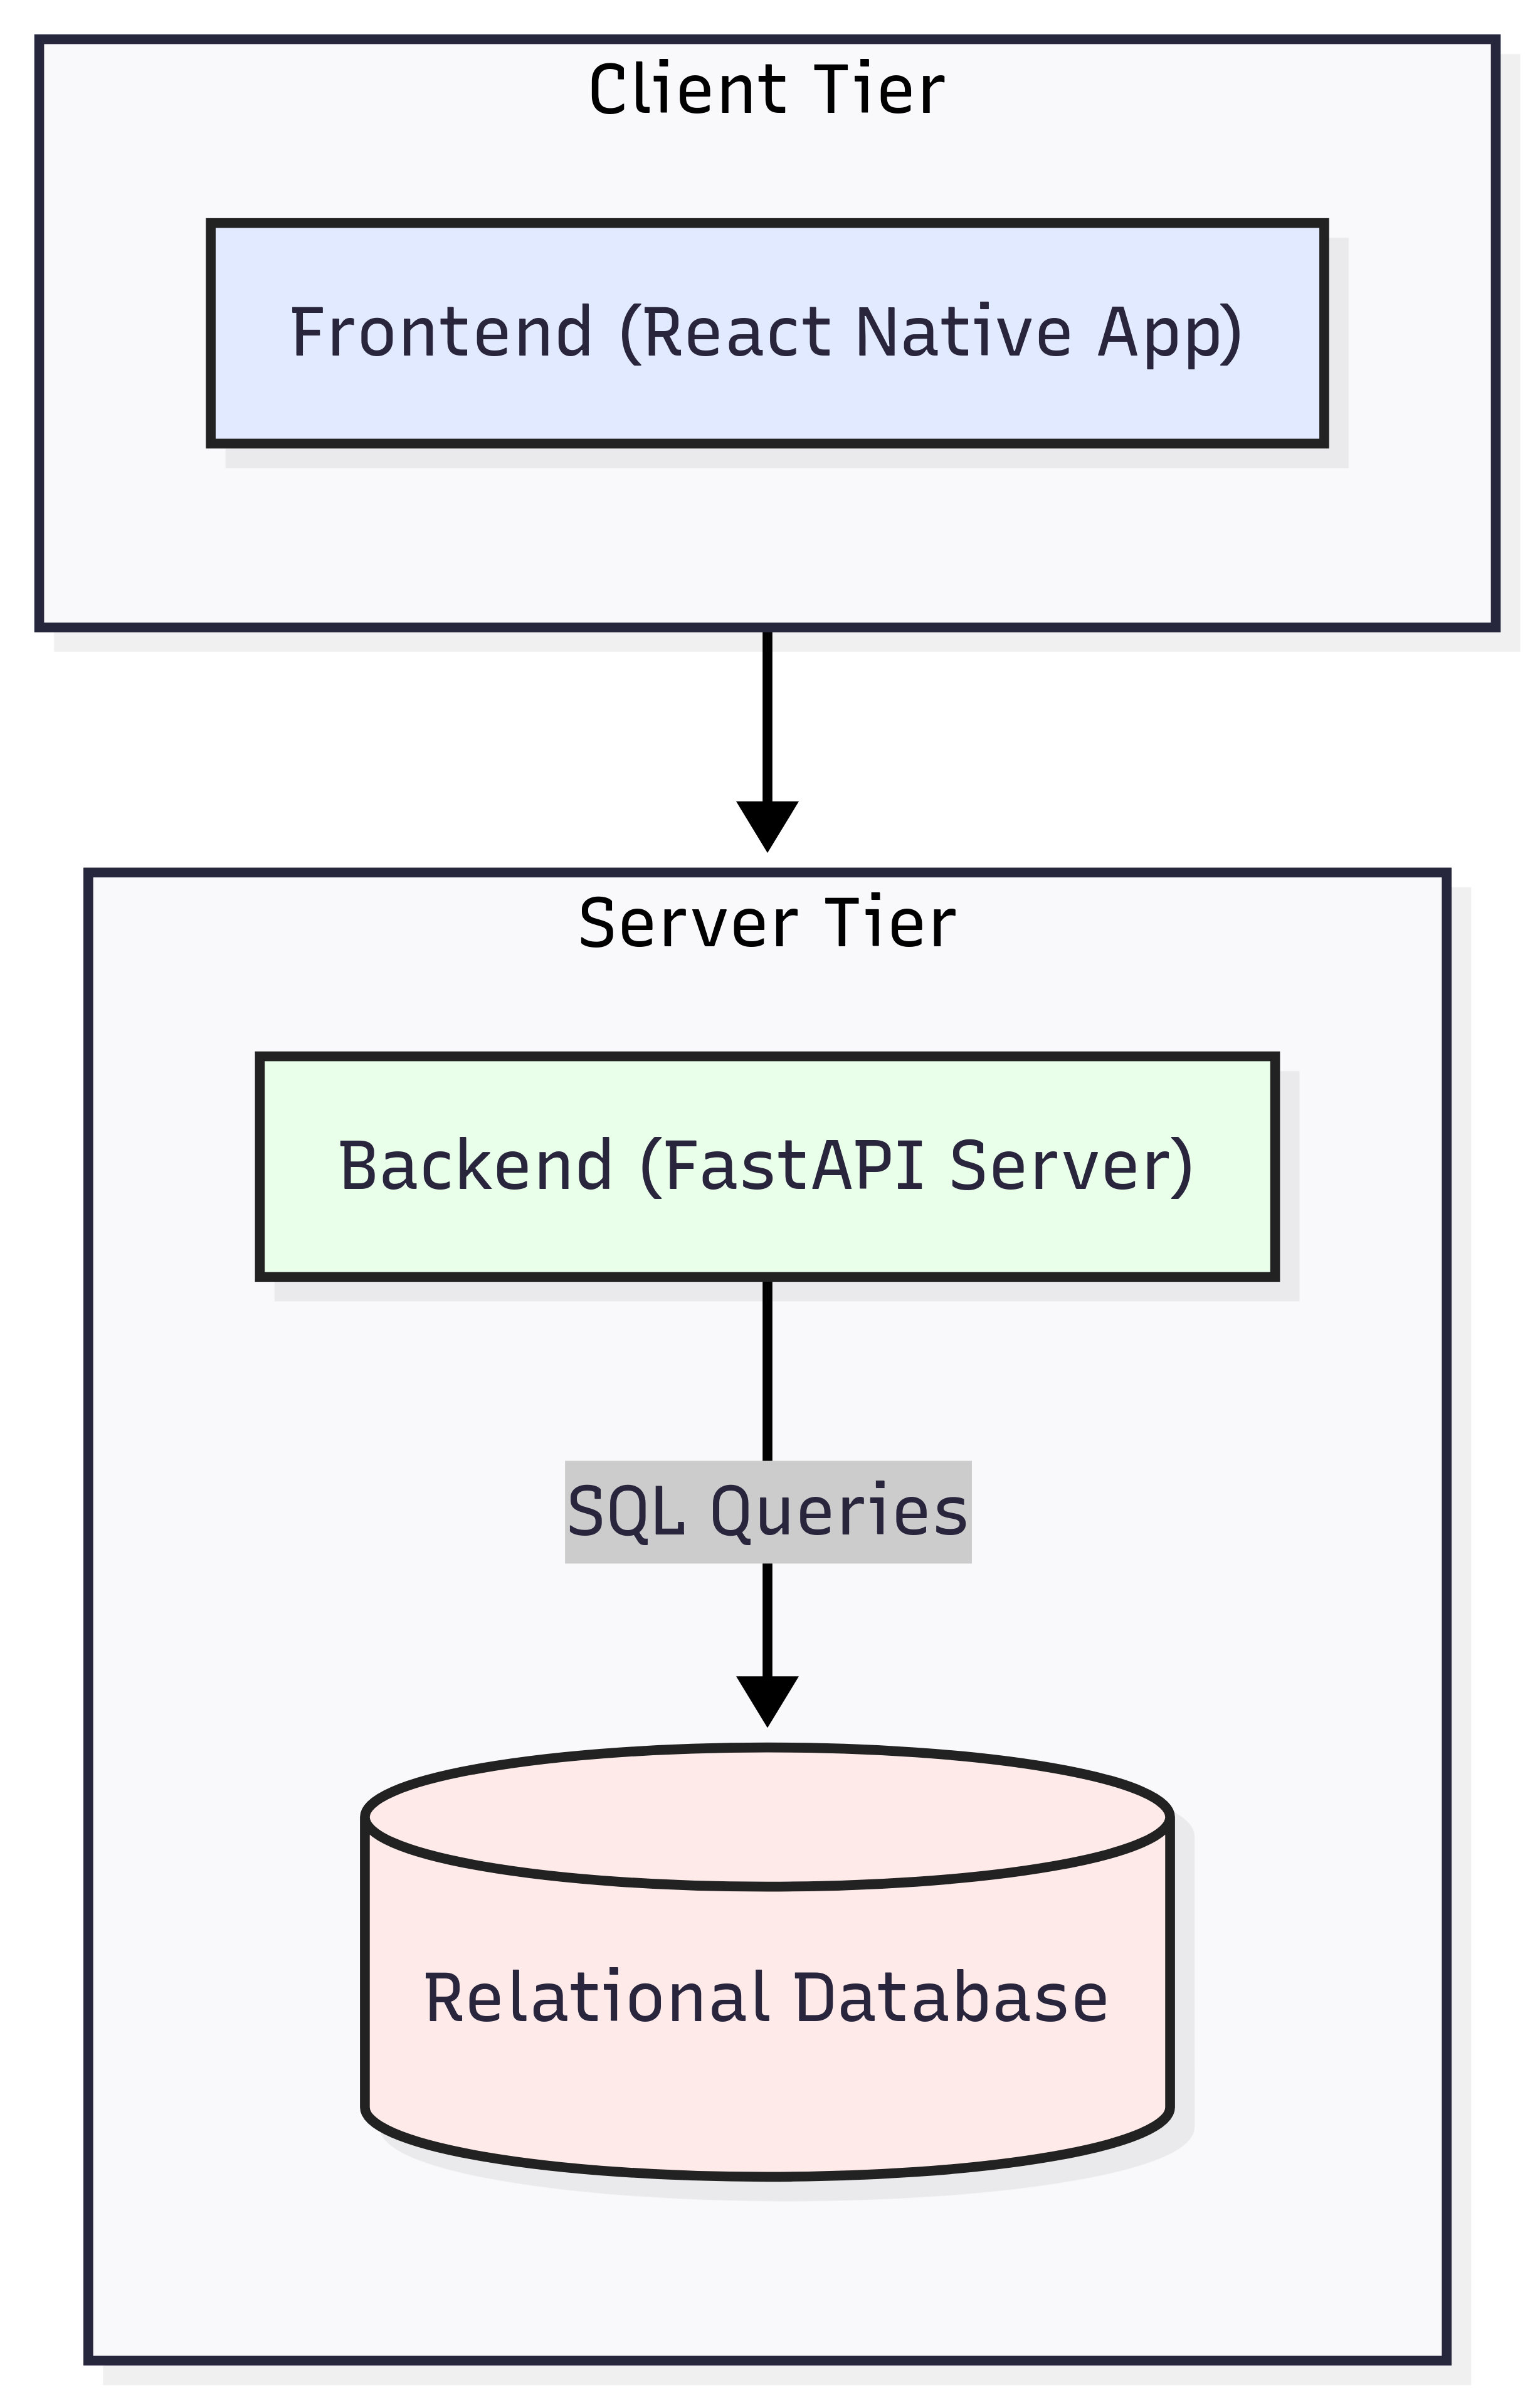
\includegraphics[width=0.9\columnwidth]{system_architecture.png}
  \caption{System architecture of TripSync: frontend, backend, and database.}
  \label{fig:system_architecture}
\end{figure}

\subsection{User Profile System}

The user profile system serves as the foundation for all platform interactions, incorporating both basic user information and institutional verification mechanisms. Each profile includes essential identification information such as name, username, college name, and course/year details, along with optional elements including profile pictures, contact numbers, and alternate email addresses.

The verification process requires validation through student ID or institutional email systems, ensuring that all users are legitimate students from recognized institutions. This verification mechanism creates the trusted environment necessary for safe transportation sharing and meaningful academic collaboration.

Profile completeness algorithms encourage users to provide comprehensive information, which enhances matching accuracy for both transportation and academic partnerships. The system maintains privacy controls that allow users to selectively share information based on interaction context and user preferences.

\subsection{Commute Module}

The commute module represents the core transportation coordination functionality, featuring an intelligent carpool finder that matches students traveling from and to similar locations. The system analyzes route patterns, timing preferences, and user ratings to optimize matches that satisfy both convenience and safety requirements.

Users can create new rides by specifying source and destination locations, preferred departure times, available seats, and any specific requirements or preferences. The ride creation interface integrates with mapping services to provide accurate location selection and route optimization.

The join ride functionality allows students to search for existing rides based on their travel requirements. Advanced filtering options include departure time windows, maximum walking distances to pickup points, and preferred user ratings or verification levels.

Safety features are integrated throughout the commute module, including verified profile requirements, rating systems, and emergency contact protocols. Real-time tracking during active rides provides additional security and accountability for all participants.

\subsection{Community Module}

The community module creates dedicated digital spaces for academic collaboration and knowledge sharing among students from different academic levels. The system provides college-specific chat rooms and groups that facilitate both formal and informal educational interactions.

Research paper exchange functionality allows students to share academic work, seek feedback, and collaborate on joint projects. The system includes version control and collaborative editing features that support academic writing partnerships between junior and senior students.

Mentorship coordination tools enable senior students to offer guidance and support to junior students across various academic and professional development areas. The platform includes structured mentorship program features with goal setting, progress tracking, and outcome assessment capabilities.

Placement guidance and career development resources are integrated into the community module, allowing students to share internship opportunities, interview experiences, and professional networking connections. This creates a comprehensive support system that extends beyond immediate academic needs.

\subsection{Additional Platform Features}

The notification system provides real-time updates for new ride opportunities, community discussions, academic collaboration requests, and system announcements. Smart notification algorithms prevent information overload while ensuring users receive relevant and timely updates.

The cost-splitting calculator automatically determines fair cost distribution for shared rides based on distance traveled, tolls, fuel costs, and other relevant factors. The system provides transparent calculations that all participants can review and approve.

A comprehensive rating and review system enables users to evaluate their experiences with both transportation partners and academic collaborators. This bidirectional feedback system maintains platform quality and helps users make informed decisions about future interactions.

Integration with external services includes mapping and navigation APIs for route optimization, payment systems for transaction management, and institutional databases for verification and administrative oversight.

\section{Technology Stack}

TripSync employs a modern, scalable technology stack designed to support cross-platform mobile deployment while ensuring robust backend performance and data management. The technology choices prioritize user experience, system reliability, and development efficiency while maintaining security and privacy standards appropriate for educational environments.

\subsection{Frontend Development}

The frontend utilizes React Native with Expo framework for cross-platform mobile application development. This technology choice enables simultaneous deployment to both iOS and Android platforms while maintaining native performance characteristics and access to device-specific features such as GPS, camera, and push notifications.

React Native's component-based architecture supports the modular design approach required for TripSync's diverse functionality, enabling efficient code reuse across different platform features. The framework's hot reloading capabilities accelerate development cycles and support rapid prototyping and testing.

Expo's managed workflow provides access to essential mobile APIs including maps, location services, notifications, and camera functionality without requiring native code development. The framework's over-the-air update capabilities enable rapid deployment of feature updates and bug fixes without requiring app store approval processes.

\subsection{Backend Architecture}

The backend employs Node.js with Express framework to create a RESTful API architecture that supports scalable, maintainable server-side operations. This technology stack provides excellent performance for real-time features while maintaining simplicity for standard CRUD operations.

Express middleware integration supports authentication, request validation, rate limiting, and security features essential for protecting student data and maintaining platform integrity. The framework's extensibility enables integration with various third-party services and APIs required for platform functionality.

Real-time communication features utilize WebSocket technology to support instant messaging, live ride coordination, and push notifications. This ensures responsive user experiences for time-sensitive interactions such as ride coordination and emergency communications.

\subsection{Database Management}

The platform employs a hybrid database approach utilizing both MongoDB for flexible document storage and PostgreSQL for structured relational data management. MongoDB handles user profiles, community content, and activity logs where schema flexibility is beneficial, while PostgreSQL manages ride coordination, financial transactions, and institutional data requiring ACID compliance.

This dual-database approach optimizes performance and data integrity while providing the flexibility needed for diverse data types and access patterns. Database selection is transparent to application logic through abstraction layers that enable future migration or scaling decisions.

Data backup and replication strategies ensure high availability and disaster recovery capabilities essential for maintaining continuous service availability for educational institutions and their students.

\subsection{Authentication and Security}

JSON Web Token (JWT) implementation provides secure, stateless authentication that scales efficiently across distributed systems. The authentication system integrates with college email verification processes to ensure institutional affiliation while maintaining user privacy.

Advanced security measures include encryption of sensitive data, secure communication protocols, and comprehensive input validation to prevent common security vulnerabilities. Regular security audits and penetration testing ensure ongoing platform security.

Privacy protection features include data anonymization options, granular permission controls, and compliance with educational privacy regulations such as FERPA and international data protection standards.

\subsection{Integration Services}

Mapping and navigation services utilize Ola Maps SDK and Google Maps API to provide accurate location services, route optimization, and real-time navigation support. These integrations ensure reliable transportation coordination while providing users with familiar navigation interfaces.

Payment processing integration supports secure financial transactions for ride cost sharing, with multiple payment methods including UPI, credit cards, and digital wallets. The system ensures PCI compliance and maintains transaction security throughout the payment process.

Institutional integration APIs enable connection with college management systems for student verification, course enrollment data, and administrative reporting. These integrations support platform administration while maintaining appropriate data privacy boundaries.

\section{Methodology}

The TripSync platform implementation follows a comprehensive methodology that encompasses user onboarding, feature utilization, and continuous improvement processes. This methodology ensures systematic user engagement while maintaining security, usability, and educational value throughout all platform interactions.

\subsection{User Registration and Verification Process}

The onboarding process begins with user registration requiring institutional email addresses and student identification verification. Students provide basic profile information including full name, student ID number, course of study, academic year, and institutional affiliation. Optional information includes profile pictures, phone numbers, and brief biographical descriptions.

Email verification occurs through automated messages sent to institutional email addresses, requiring users to confirm their identity through secure links. Student ID verification involves document upload and administrative review to ensure legitimate student status. This dual verification approach creates a trusted user base while maintaining reasonable onboarding efficiency.

Profile completion prompts guide users through providing additional information that enhances platform functionality, including transportation preferences, academic interests, and collaboration availability. The system provides privacy controls that enable users to selectively share information based on specific interaction contexts.

\subsection{Ride Coordination Workflow}

The transportation coordination process begins with route specification where users enter source and destination locations using integrated mapping interfaces. The system analyzes the specified routes to identify potential matches with existing rides or users seeking transportation to similar destinations.

Advanced matching algorithms consider multiple factors including geographical proximity, timing preferences, user ratings, gender preferences for safety, and compatibility indicators based on academic programs or interests. The system presents ranked matching options with detailed information about potential ride partners and trip logistics.

Ride confirmation requires mutual agreement between ride creators and joiners, with automated cost-sharing calculations based on distance, fuel costs, tolls, and wear-and-tear factors. The system generates detailed trip summaries including pickup and drop-off locations, timing, cost distribution, and participant contact information.

Safety protocols include pre-trip verification checks, real-time location tracking during active trips, emergency contact systems, and post-trip feedback collection. These measures ensure user safety while providing accountability mechanisms for all participants.

\subsection{Academic Collaboration Framework}

The community engagement process provides multiple pathways for academic collaboration including research paper sharing, mentorship connections, study group formation, and project partnerships. Users specify their academic interests, expertise areas, and collaboration preferences to enable intelligent matching with suitable partners.

Mentorship coordination involves structured processes for connecting senior students with juniors seeking guidance in specific academic or professional development areas. The system includes goal-setting frameworks, progress tracking mechanisms, and outcome assessment tools to ensure meaningful mentoring relationships.

Research collaboration tools support document sharing, version control, collaborative editing, and communication management for joint academic projects. Integration with popular academic tools enhances functionality while maintaining platform coherence and user experience consistency.

\subsection{Continuous Improvement and Analytics}

User feedback collection occurs through multiple mechanisms including post-interaction ratings, periodic satisfaction surveys, and feature usage analytics. This data informs platform improvements and helps identify successful interaction patterns that can be promoted and replicated.

Performance monitoring tracks key metrics including ride completion rates, academic collaboration success, user retention, cost savings achieved, and environmental impact measurements. Regular analysis of these metrics guides feature development priorities and user engagement strategies.

Administrative reporting provides institutional partners with aggregated usage statistics, safety metrics, and educational outcome indicators while maintaining individual user privacy. These reports support program evaluation and institutional decision-making regarding platform adoption and promotion.

\section{Expected Outcomes}

TripSync implementation is anticipated to generate significant positive impacts across multiple dimensions of student experience, institutional efficiency, and environmental sustainability. These expected outcomes are based on literature review findings, similar platform performance data, and preliminary user research conducted during platform development.

\subsection{Economic Benefits for Students}

Primary economic benefits include substantial reduction in individual transportation costs through effective ride-sharing coordination. Analysis indicates potential cost savings of 40-60\% compared to individual transportation or commercial ride-sharing services, with average monthly savings of Rs.1500-2400 per active user.

Secondary economic benefits emerge from increased access to academic resources, mentorship opportunities, and peer support networks that can improve academic performance and reduce academic support costs. Enhanced placement guidance and career networking may also contribute to improved post-graduation employment outcomes.

Cost distribution transparency and automated calculation features ensure fair expense sharing while reducing conflicts and improving user satisfaction with ride-sharing arrangements. These features contribute to sustained platform usage and community growth.

\subsection{Safety and Security Improvements}

The verified student-only ecosystem significantly enhances transportation safety compared to commercial ride-sharing platforms. Institutional verification, peer rating systems, and community accountability mechanisms create multiple layers of safety assurance for platform users.

Emergency contact systems, real-time location tracking, and institutional oversight provide additional security features specifically designed for educational environments. These features address parental and institutional concerns while enabling student independence and mobility.

Gender-specific safety features including same-gender ride options and enhanced verification for cross-gender interactions address specific safety concerns while maintaining inclusive platform access for all students.

\subsection{Academic and Social Collaboration Enhancement}

Structured academic collaboration tools are expected to increase meaningful interactions between junior and senior students by 200-300\% compared to informal networking approaches. These interactions contribute to improved learning outcomes, enhanced peer support, and stronger institutional community development.

Mentorship program success rates are anticipated to improve through systematic matching, goal-setting, and progress tracking features. Early adopter feedback indicates high satisfaction with structured mentorship approaches compared to informal arrangements.

Research collaboration and academic paper sharing features may contribute to increased student research productivity, improved academic writing skills, and enhanced preparation for graduate education or research careers.

\subsection{Environmental Impact}

Transportation consolidation through ride-sharing is expected to reduce individual vehicle trips by 25-30\% among active users, contributing to decreased traffic congestion around educational institutions and reduced carbon emissions from student commuting.

Environmental impact tracking and reporting features raise student awareness of sustainability issues while providing institutions with data to support environmental initiatives and reporting requirements.

Gamification elements related to sustainable transportation choices may amplify environmental benefits by encouraging continued eco-friendly behavior among platform users.

\subsection{Institutional Benefits}

Administrative efficiency improvements include reduced coordination burden for student transportation, enhanced visibility into student commuting patterns, and systematic data collection regarding student collaboration and engagement activities.

Safety incident reduction and improved emergency response capabilities contribute to institutional risk management and student welfare objectives. Comprehensive reporting features support institutional accountability and program evaluation requirements.

Enhanced student satisfaction and community development may contribute to improved retention rates, stronger alumni networks, and enhanced institutional reputation among prospective students and their families.

\section{Future Scope}

The long-term development roadmap for TripSync encompasses technological enhancements, feature expansions, and platform scaling initiatives that will significantly extend its impact and utility within educational environments. These future developments are designed to leverage emerging technologies while responding to evolving student needs and institutional requirements.

\subsection{Artificial Intelligence Integration}

AI-based ride matching optimization represents a major enhancement opportunity that will improve matching accuracy and user satisfaction through machine learning algorithms. These systems will analyze historical usage patterns, user preferences, successful interaction indicators, and external factors such as weather and traffic conditions to provide increasingly accurate ride and academic collaboration matches.

Predictive analytics capabilities will enable proactive ride suggestions based on user schedules, historical patterns, and institutional event calendars. Natural language processing integration may enhance community interaction features and provide intelligent content recommendations for academic collaboration.

Intelligent scheduling algorithms will optimize ride timing and route coordination to minimize total travel time while maximizing passenger convenience. These features will become increasingly sophisticated as the platform accumulates usage data and user feedback.

\subsection{Payment System Integration}

Comprehensive digital payment integration will streamline financial transactions through UPI, digital wallet, and traditional payment method support. Automated payment processing will eliminate manual cost-sharing negotiations while ensuring transparent, fair expense distribution among ride participants.

Subscription-based payment models may provide users with premium features including priority matching, enhanced safety features, and expanded community access. These models will support platform sustainability while providing additional value for frequent users.

Integration with institutional financial systems may enable seamless payment processing through student accounts or institutional financial aid programs, reducing barriers to platform adoption and usage.

\subsection{Inter-College Networking Expansion}

Platform expansion beyond individual institutions will create regional student networks that enhance collaboration opportunities and transportation efficiency across multiple educational institutions. This expansion requires development of inter-institutional verification systems and enhanced security protocols.

Cross-institutional academic collaboration features will enable research partnerships, joint projects, and knowledge sharing among students from different colleges and universities. These features may contribute to enhanced educational outcomes and broader academic networking opportunities.

Regional transportation hubs and long-distance ride coordination will address student travel needs for internships, conferences, and inter-institutional academic activities. Enhanced route optimization and safety protocols will be essential for these expanded services.

\subsection{Gamification and Engagement Enhancement}

Comprehensive gamification systems will reward environmentally conscious transportation choices, active community participation, and positive peer interactions. These systems will include achievement badges, leaderboards, and institutional recognition programs that encourage sustained platform engagement.

Social impact tracking will quantify and celebrate user contributions to environmental sustainability, peer support, and community development. Public recognition of positive contributions may enhance user motivation and platform community development.

Competitive elements between institutions may encourage broader platform adoption while fostering healthy inter-institutional relationships and collaboration. These features require careful design to maintain positive community dynamics.

\subsection{Advanced Analytics and Reporting}

Sophisticated analytics platforms will provide institutions with detailed insights into student transportation patterns, collaboration success rates, and community engagement metrics. These analytics will support evidence-based decision making regarding transportation policies, academic support programs, and campus development initiatives.

Longitudinal outcome tracking will assess platform impact on academic performance, student satisfaction, graduation rates, and post-graduation success indicators. This research will contribute to educational technology literature while supporting platform improvement and adoption.

Integration with institutional research systems will enable comprehensive analysis of platform impact on broader educational outcomes and institutional effectiveness measures. These capabilities will support platform evaluation and continuous improvement initiatives.

\section{Conclusions}

TripSync represents a comprehensive solution to interconnected challenges in student transportation and academic collaboration within higher education environments. Through careful integration of commute-sharing functionality with structured academic collaboration features, the platform addresses critical gaps in existing educational technology while providing measurable benefits across multiple dimensions of student experience.

The literature review demonstrates substantial empirical support for the platform's core design principles, particularly the integration of service-learning management concepts with peer-to-peer transportation sharing. Research consistently shows that structured peer interactions, guided by clear protocols and supported by appropriate technology, significantly enhance both academic and social outcomes for students. TripSync leverages these insights while addressing practical transportation challenges that affect daily student life.

The platform's technological architecture provides a scalable, secure foundation for supporting diverse student needs while maintaining the trust and safety essential for educational environments. The choice of modern, cross-platform development technologies ensures broad accessibility while enabling rapid feature development and deployment. Integration capabilities support institutional requirements while maintaining student privacy and autonomy.

Expected outcomes across economic, safety, academic, and environmental dimensions demonstrate TripSync's potential for significant positive impact on student life and institutional effectiveness. Cost reduction of 40-60\% for transportation, enhanced safety through verified user networks, increased academic collaboration, and measurable environmental benefits collectively justify the platform development and deployment investment.

Future development opportunities, including AI integration, payment system enhancements, and inter-institutional expansion, position TripSync for continued relevance and impact as student needs and educational environments evolve. The platform's modular architecture and comprehensive data collection capabilities provide the foundation for these advanced features while supporting ongoing research and improvement initiatives.

The integration of transportation coordination with academic collaboration represents an innovative approach to educational technology that recognizes the interconnected nature of student needs and experiences. By addressing both practical logistics and educational outcomes through a unified platform, TripSync demonstrates the potential for technology solutions that enhance rather than fragment the student experience.

TripSync's development and implementation provide valuable contributions to educational technology research while offering immediate practical benefits for students and institutions. The platform's success will depend on sustained engagement from educational institutions, continued technological innovation, and responsiveness to evolving student needs and preferences. Nevertheless, the strong theoretical foundation, comprehensive feature set, and clear implementation pathway position TripSync as a significant advancement in student-centered educational technology.

\begin{thebibliography}{99}
\bibitem{ref1} "Student collaboration and academic engagement in higher education," \emph{ScienceDirect}. [Online]. Available: https://www.sciencedirect.com/science/article/pii/S2405844025008345. [Accessed: Aug. 22, 2025].

\bibitem{ref2} "Student project hub management system," \emph{IRJ Web}. [Online]. Available: https://www.irjweb.com/STUDENT\%20PROJECT\%20HUB.pdf. [Accessed: Aug. 22, 2025].

\bibitem{ref3} "Web-based student project management system: A TETFund institution based research report," \emph{International Journal of Current Science Research and Review}. [Online]. Available: https://ijcsrr.org/web-based-student-project-management-system-a-tetfund-institution-based-research-report/. [Accessed: Aug. 22, 2025].

\bibitem{ref4} "Digital transformation in educational project management," \emph{International Journal of Creative Research Thoughts}, 2024. [Online]. Available: https://www.ijcrt.org/papers/IJCRT24A5413.pdf. [Accessed: Aug. 22, 2025].

\bibitem{ref5} "Faculty engagement and student collaboration in higher education," \emph{University of New Hampshire Scholars' Repository}. [Online]. Available: https://scholars.unh.edu/cgi/viewcontent.cgi?article=1716\&context=faculty\_pubs. [Accessed: Aug. 22, 2025].

\bibitem{ref6} "Student engagement and collaboration technologies in education," \emph{ERIC Educational Resources Information Center}. [Online]. Available: https://files.eric.ed.gov/fulltext/EJ1133851.pdf. [Accessed: Aug. 22, 2025].

\bibitem{ref7} "Vishwa connect: A ride sharing mobile application," \emph{Journal of Research in Applied Science, Engineering and Technology}. [Online]. Available: https://www.jjraset.com/best-journal/vishwa-connect-a-ride-sharing-mobile-application1. [Accessed: Aug. 22, 2025].

\bibitem{ref8} "Sustainable transportation solutions for university communities," \emph{MDPI Sustainability}, vol. 16, no. 14, 2024. [Online]. Available: https://www.mdpi.com/2071-1050/16/14/58947. [Accessed: Aug. 22, 2025].

\bibitem{ref9} "Mobile application development for student transportation," \emph{IEEE Xplore Digital Library}. [Online]. Available: https://ieeexplore.ieee.org/stamp/stamp.jsp?tp=\&arnumber=792101212. [Accessed: Aug. 22, 2025].

\bibitem{ref10} "Technology-enhanced student engagement and collaboration," \emph{Oxford Academic Transportation Science \& Engineering}, vol. 6, no. 2, 2023. [Online]. Available: https://academic.oup.com/tse/article/6/2/tdad025/7161803?utm\_source=chatgpt.com\&login=false17. [Accessed: Aug. 22, 2025].

\bibitem{ref11} "Digital platforms for academic collaboration in higher education," \emph{IEEE Xplore Digital Library}. [Online]. Available: https://ieeexplore.ieee.org/document/708391023. [Accessed: Aug. 22, 2025].

\bibitem{ref12} "Student-centric mobile applications for campus management," \emph{IEEE Xplore Digital Library}. [Online]. Available: https://ieeexplore.ieee.org/document/650312428. [Accessed: Aug. 22, 2025].

\bibitem{ref13} "Integrated solutions for campus communication and collaboration," \emph{IEEE Xplore Digital Library}. [Online]. Available: https://ieeexplore.ieee.org/document/882172233. [Accessed: Aug. 22, 2025].

\bibitem{ref14} "Smart campus technologies and student engagement systems," \emph{IEEE Xplore Digital Library}. [Online]. Available: https://ieeexplore.ieee.org/document/547845338. [Accessed: Aug. 22, 2025].

\bibitem{ref15} "Campus mobility solutions and ride-sharing platforms," \emph{IEEE Xplore Digital Library}. [Online]. Available: https://ieeexplore.ieee.org/document/800116043. [Accessed: Aug. 22, 2025].

\bibitem{ref16} "Car pooling system development and implementation," \emph{JUIT Institutional Repository}. [Online]. Available: http://www.ir.juit.ac.in:8080/jspui/bitstream/123456789/6680/1/Car\%20Pooling\%20System.pdf64646464. [Accessed: Aug. 22, 2025].

\bibitem{ref17} "RTG carpooling application design and development," \emph{JUIT Institutional Repository}. [Online]. Available: http://ir.juit.ac.in:8080/jspui/bitstream/123456789/7130/1/RTG\%20Carpooling\%20Application.pdf69. [Accessed: Aug. 22, 2025].
\end{thebibliography}

\end{document}